%!TEX root = ../thesis.tex

\thispagestyle{myheadings}

\graphicspath{{Body/Figures/Wa/Datasets/60h/BunchNum/}{Body/Figures/Wa/Datasets/HighKick/BunchNum/}{Body/Figures/Wa/Datasets/9d/BunchNum/}{Body/Figures/Wa/Datasets/Endgame/BunchNum/}{Body/Figures/Wa/Datasets/60h/SingleIteration/FitStartScans/}{Body/Figures/Wa/Datasets/HighKick/SingleIteration/FitStartScans/}{Body/Figures/Wa/Datasets/9d/SingleIteration/FitStartScans/}{Body/Figures/Wa/Datasets/Endgame/SingleIteration/FitStartScans/}{Body/Figures/Wa/Datasets/60h/SingleIteration/FitEndScans/}{Body/Figures/Wa/Datasets/HighKick/SingleIteration/FitEndScans/}{Body/Figures/Wa/Datasets/9d/SingleIteration/FitEndScans/}{Body/Figures/Wa/Datasets/Endgame/SingleIteration/FitEndScans/}{Body/Figures/Wa/Datasets/60h/EnergyThreshold/}{Body/Figures/Wa/Datasets/HighKick/EnergyThreshold/}{Body/Figures/Wa/Datasets/9d/EnergyThreshold/}{Body/Figures/Wa/Datasets/Endgame/EnergyThreshold/}{Body/Figures/Wa/Datasets/60h/RandSeeds/}{Body/Figures/Wa/Datasets/HighKick/RandSeeds/}{Body/Figures/Wa/Datasets/9d/RandSeeds/}{Body/Figures/Wa/Datasets/Endgame/RandSeeds/}{Body/Figures/Wa/Datasets/60h/SingleIteration/CaloFits/}{Body/Figures/Wa/Datasets/HighKick/SingleIteration/CaloFits/}{Body/Figures/Wa/Datasets/9d/SingleIteration/CaloFits/}{Body/Figures/Wa/Datasets/Endgame/SingleIteration/CaloFits/}{Body/Figures/Wa/Datasets/60h/SingleIteration/SingleFits/}{Body/Figures/Wa/Datasets/HighKick/SingleIteration/SingleFits/}{Body/Figures/Wa/Datasets/9d/SingleIteration/SingleFits/}{Body/Figures/Wa/Datasets/Endgame/SingleIteration/SingleFits/}{Body/Figures/Wa/Datasets/ComparisonPlots/CaloFits/}{Body/Figures/Wa/Datasets/ComparisonPlots/FitStartScan/}{Body/Figures/Wa/Miscellaneous/}}




\section{Fit results}
\label{sec:fit_results}


\figref{fig:moduloPlots} shows fits to the four Run~1 precession frequency analysis datasets for single random seeds. \tabref{tab:DatasetFitResults} gives all fit parameters and their errors. In each dataset case the \chisq/NDF is acceptable as evidenced by the p-value included in the table results. Fit pulls and the FFT of the fit residuals for the 60h dataset are provided in Figure~\ref{fig:fitResiduals_60h}. As shown all structure has been eliminated within the fit residuals implying that all effects in the data have properly been accounted for in the fit function. The same checks were made for the HighKick, 9d, and Endgame datasets and in each case no residual structure remained. \appref{app:CorrelationMatrices} provides the correlation matrices for the various datasets. The only fit parameter that is significantly correlated with $R$ is the \gmtwo phase in all datasets. This increases the confidence in the \wa extraction, as effects in the data which might potentially be mis-modeled will only weakly correlate with the final fitted $R$ value. The various different CBO parameters are self-correlated to different degrees depending on the parameter and the dataset that is being fit. Typically either the phases and frequencies are correlated, or the lifetimes and amplitudes. 

The \gmtwo phases for the different datasets showed small differences, due primarily to upstream beam adjustments before injection into the storage ring. Similarly, slightly different asymmetries can be attributed to very small acceptance differences in the stored beams. As described in \secref{subsec:lostmuons}, the value for \K was determined and fixed from a T-Method fit to the data. The values themselves don't directly correspond to the level of losses, as each dataset has it's own loss function $L(t)$.


\begin{figure}
\centering
    \begin{subfigure}[]{0.45\textwidth}
        \centering
        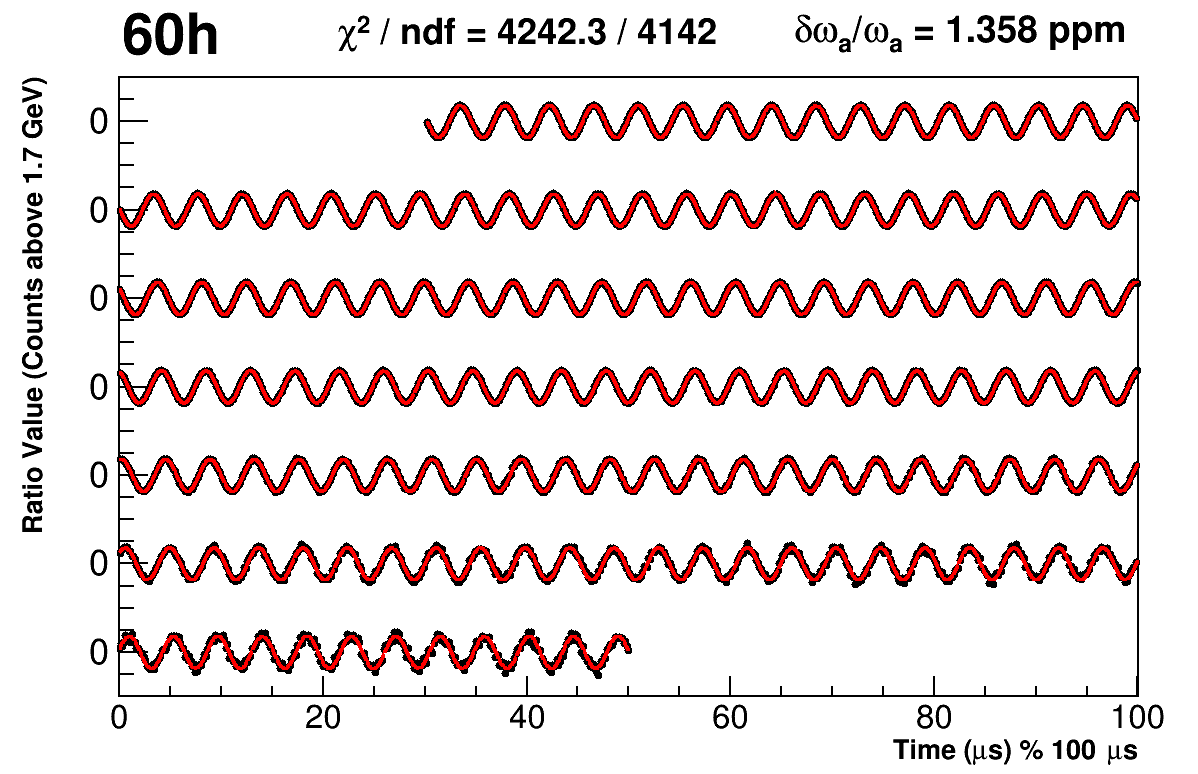
\includegraphics[width=\textwidth]{fullRatio_moduloPlot_noStats_60h}
        % \caption{60h dataset.}
    \end{subfigure}% %you need this % here to add spacing between subfigures
    \begin{subfigure}[]{0.45\textwidth}
        \centering
        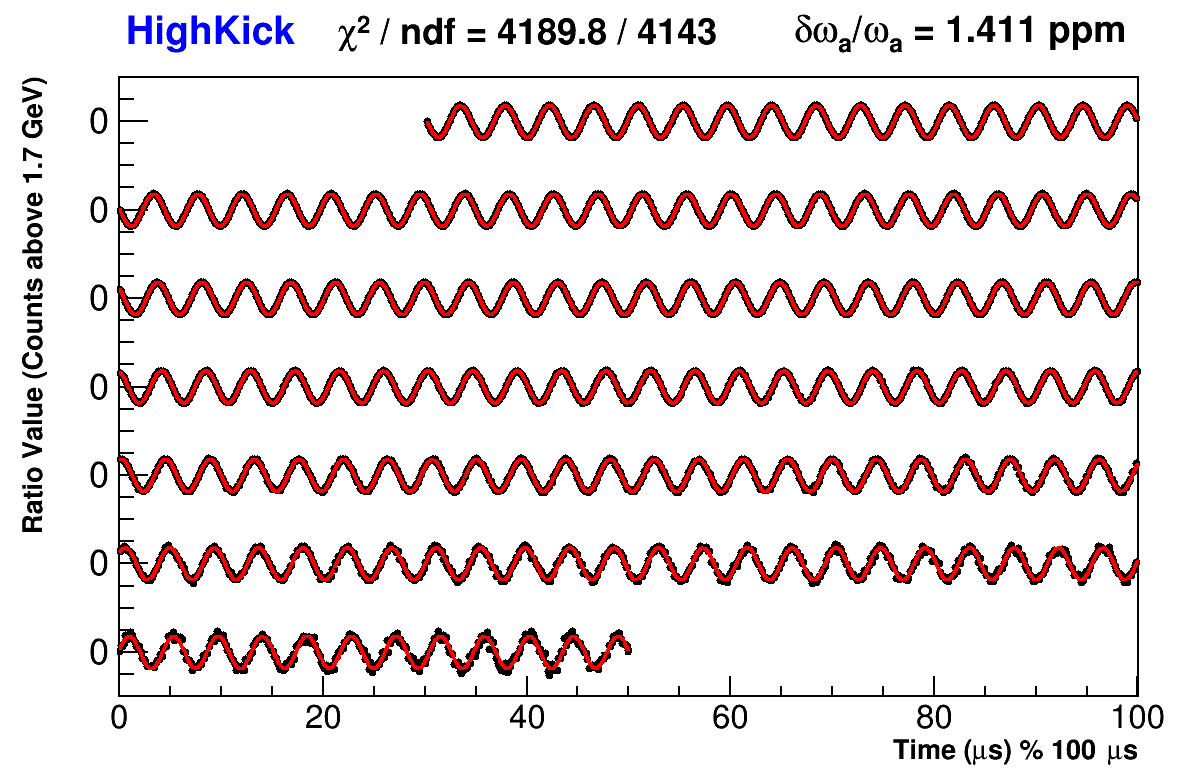
\includegraphics[width=\textwidth]{fullRatio_moduloPlot_noStats_HighKick}
        % \caption{HighKick dataset.}
    \end{subfigure}
    \vspace{4mm}
    \begin{subfigure}[]{0.45\textwidth}
        \centering
        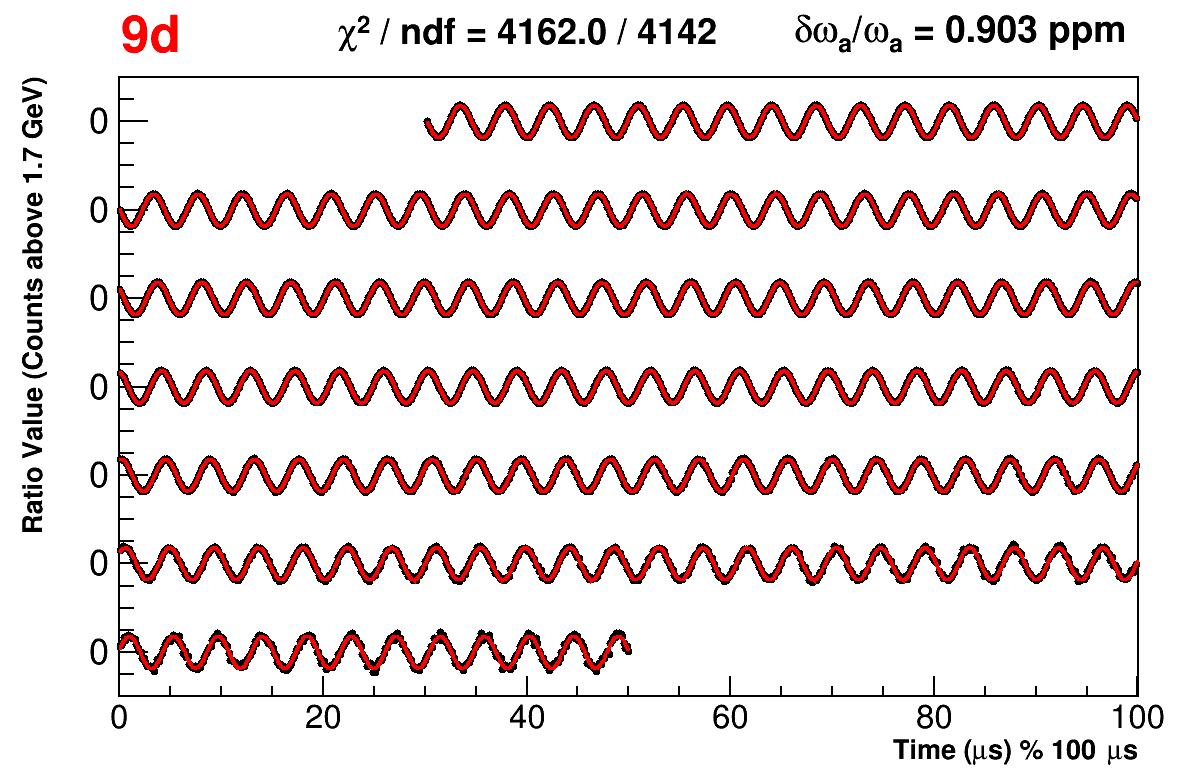
\includegraphics[width=\textwidth]{fullRatio_moduloPlot_noStats_9d}
        % \caption{9d dataset.}
    \end{subfigure}% %you need this % here to add spacing between subfigures
    \begin{subfigure}[]{0.45\textwidth}
        \centering
        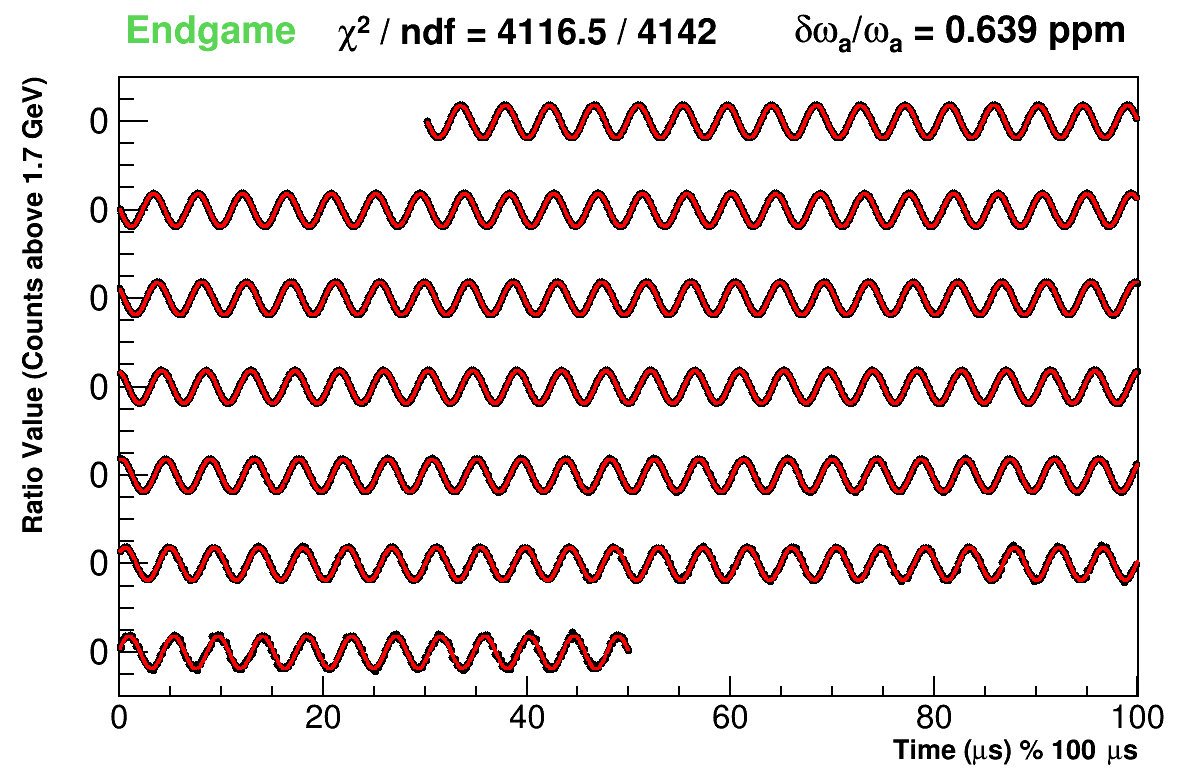
\includegraphics[width=\textwidth]{fullRatio_moduloPlot_noStats_Endgame}
        % \caption{Endgame dataset.}
    \end{subfigure}
\caption[Single random seed fits to calorimeter summed data of Run~1 precession frequency analysis datasets]{Single random seed fits to calorimeter summed data of Run~1 precession frequency analysis datasets. Data is in black and the fits are in red. The x axis is in units of \mus{} modulo \mus{100}, with successive portions of the data points and fit shifted downwards on the plot. The fit ranges from 30.2--\mus{650}. Dataset names are given in the upper left corners of the figures, alongside the \chisq per degree of freedom and relative error on \wa or $R$.}
\label{fig:moduloPlots}
\end{figure}



% \afterpage{
\clearrow
\begin{landscape}
\begin{table}
\centering
\small
% \setlength\tabcolsep{10pt}
\renewcommand{\arraystretch}{1.2}
% \begin{tabular*}{\linewidth}{@{\extracolsep{\fill}}l|cc|cc|cc|cc}
% \begin{tabular*}{\linewidth}{@{\extracolsep{\fill}}l|>{\rowmac}c>{\rowmac}c|>{\rowmac}c>{\rowmac}c|>{\rowmac}c>{\rowmac}c|>{\rowmac}c>{\rowmac}c<{\clearrow}}
\begin{tabular*}{\linewidth}{@{\extracolsep{\fill}}l|>{\rowmac}l>{\rowmac}l|>{\rowmac}l>{\rowmac}l|>{\rowmac}l>{\rowmac}l|>{\rowmac}l>{\rowmac}l<{\clearrow}}
% \begin{tabular*}{\linewidth}{@{\extracolsep{\fill}}l|>{\rowmac}S[table-format=3.3]>{\rowmac}S[table-format=3.3]|>{\rowmac}S[table-format=3.3]>{\rowmac}S[table-format=3.3]|>{\rowmac}S[table-format=3.3]>{\rowmac}S[table-format=3.3]|>{\rowmac}S[table-format=3.3]>{\rowmac}S[table-format=3.3]<{\clearrow}}
  \hline
    \multicolumn{9}{c}{\textbf{Ratio Method Fit Results}} \\
  \hline\hline
 & \multicolumn{2}{c|}{60h} & \multicolumn{2}{c|}{HighKick} & \multicolumn{2}{c|}{9d} & \multicolumn{2}{c}{Endgame} \\
  \hline\hline
    $\chi^{2}$/NDF & \multicolumn{2}{c|}{$4242/4142$} & \multicolumn{2}{c|}{$4190/4143$} & \multicolumn{2}{c|}{$4162/4142$} & \multicolumn{2}{c}{$4116/4142$} \\
    p-value        & \multicolumn{2}{c|}{$0.1356$} & \multicolumn{2}{c|}{$0.3018$} & \multicolumn{2}{c|}{$0.4104$} & \multicolumn{2}{c}{$0.6079$}  \\
  \hline\hline
    Parameter & Value & Error & Value & Error & Value & Error & Value & Error \\
  \hline
    $A$                               &  $\SI{0.3637}{}$ & $\SI{4.4e-05}{}$ & $\SI{0.3632}{}$ & $\SI{4.6e-05}{}$ & $\SI{0.3639}{}$ & $\SI{2.9e-05}{}$ & $\SI{0.3686}{}$ & $\SI{2.1e-05}{}$ \\
    
    \setrow{\bfseries} 
    $R$ (ppm, blinded)                &  $\SI{-20.8479}{}$ & $\SI{1.3581}{}$ & $\SI{-17.5433}{}$ & $\SI{1.4112}{}$ & $\SI{-17.8214}{}$ & $\SI{0.9033}{}$ & $\SI{-17.5674}{}$ & $\SI{0.6393}{}$ \\
    
    $\phi$                            &  $\SI{2.091}{}$ & $\SI{2.2e-4}{}$ & $\SI{2.081}{}$ & $\SI{2.3e-4}{}$ & $\SI{2.080}{}$ & $\SI{1.5e-4}{}$ & $\SI{2.076}{}$ & $\SI{1.1e-4}{}$ \\
    
    $\omega_{cbo}$ (rad/\mus{})       &  $\SI{2.338}{}$ & $\SI{1.4e-3}{}$ & $\SI{2.599}{}$ & $\SI{6.6e-3}{}$ & $\SI{2.615}{}$ & $\SI{5.6e-3}{}$ & $\SI{2.339}{}$ & $\SI{0.8e-3}{}$ \\
    
    $\tau_{cbo}$ (\mus{})             &  $\SI{175.2}{}$ & $\SI{46.8}{}$ & $\SI{99.4}{}$ & $\SI{0}{}$ & $\SI{137.4}{}$ & $\SI{62.0}{}$ & $\SI{200.3}{}$ & $\SI{33.5}{}$ \\
    
    $A_{cbo-N} \;(\times 10^{-4})$    &  $\SI{43.1}{}$ & $\SI{5.0}{}$ & $\SI{42.8}{}$ & $\SI{9.9}{}$ & $\SI{39.3}{}$ & $\SI{9.7}{}$ & $\SI{32.3}{}$ & $\SI{2.0}{}$ \\
    
    $\phi_{cbo-N}$                    &  $\SI{-2.343}{}$ & $\SI{0.107}{}$ & $\SI{3.817}{}$ & $\SI{0.446}{}$ & $\SI{3.302}{}$ & $\SI{0.374}{}$ & $\SI{-0.710}{}$ & $\SI{0.062}{}$ \\
    
    $A_{2cbo-N} \;(\times 10^{-4})$   &  $\SI{1.9}{}$ & $\SI{1.3}{}$ & $\SI{4.9}{}$ & $\SI{4.5}{}$ & $\SI{2.2}{}$ & $\SI{2.7}{}$ & $\SI{1.2}{}$ & $\SI{0.5}{}$ \\
    
    $\phi_{2cbo-N}$                   &  $\SI{3.331}{}$ & $\SI{0.638}{}$ & $\SI{5.665}{}$ & $\SI{1.274}{}$ & $\SI{-4.936}{}$ & $\SI{1.127}{}$ & $\SI{0.322}{}$ & $\SI{0.448}{}$ \\
   
    $A_{cbo-A} \;(\times 10^{-4})$    &  $\SI{05.5}{}$ & $\SI{3.9}{}$ & $\SI{9.5}{}$ & $\SI{4.1}{}$ & $\SI{6.4}{}$ & $\SI{2.5}{}$ & $\SI{2.7}{}$ & $\SI{1.9}{}$ \\
   
    $\phi_{cbo-A}$                    &  $\SI{-0.271}{}$ & $\SI{0.737}{}$ & $\SI{-2.073}{}$ & $\SI{0.600}{}$ & $\SI{1.750}{}$ & $\SI{0.561}{}$ & $\SI{-2.825}{}$ & $\SI{0.686}{}$ \\
    
    $A_{cbo-\phi} \;(\times 10^{-4})$ &  $\SI{8.0}{}$ & $\SI{4.2}{}$ & $\SI{5.7}{}$ & $\SI{4.4}{}$ & $\SI{8.8}{}$ & $\SI{3.1}{}$ & $\SI{1.9}{}$ & $\SI{1.9}{}$ \\
    
    $\phi_{cbo-\phi}$                 &  $\SI{-1.183}{}$ & $\SI{0.533}{}$ & $\SI{1.227}{}$ & $\SI{0.920}{}$ & $\SI{4.313}{}$ & $\SI{0.415}{}$ & $\SI{-1.576}{}$ & $\SI{0.995}{}$ \\
    
    $\kappa_{loss}$                   &  $\SI{8.974}{}$ & $\SI{0}{}$ & $\SI{5.651}{}$ & $\SI{0}{}$ & $\SI{2.510}{}$ & $\SI{0}{}$ & $\SI{2.345}{}$ & $\SI{0}{}$ \\
  \hline
\end{tabular*}
\caption[Fit results for Run~1 precession frequency analysis datasets]{Fit parameters for the four Run~1 precession frequency analysis datasets for a single random seed. The bold row highlights the final fitted $R$ values and their respective errors. The 60h dataset has a different blinding to the rest. The \K parameter is fixed in each dataset fit corresponding to the 0 value in the error column, and similarly for $\tau_{cbo}$ in the fit to the HighKick dataset.}
\label{tab:DatasetFitResults}
\end{table}
\end{landscape}
% }



% \afterpage{
\begin{landscape}
\begin{figure}
\centering
    \begin{subfigure}[b]{0.45\textwidth}
        \centering
        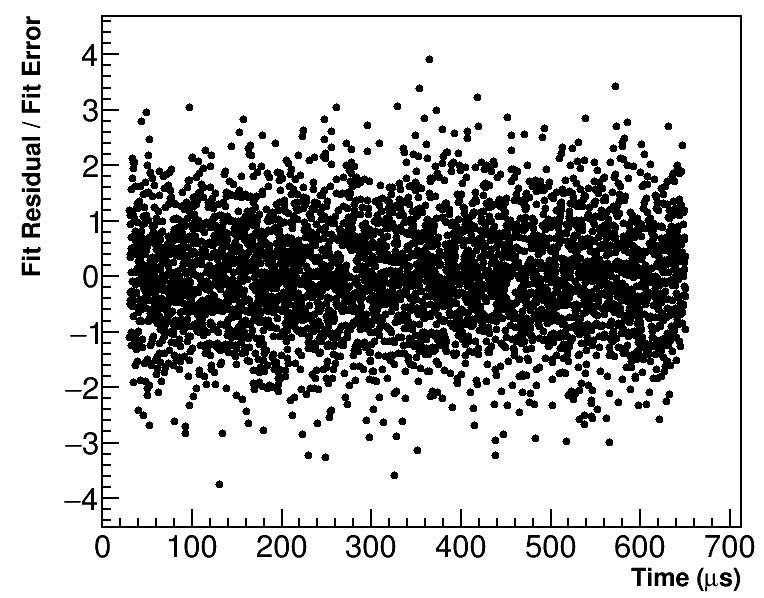
\includegraphics[width=\textwidth]{fitPull_60h}
    \vspace{4mm}
        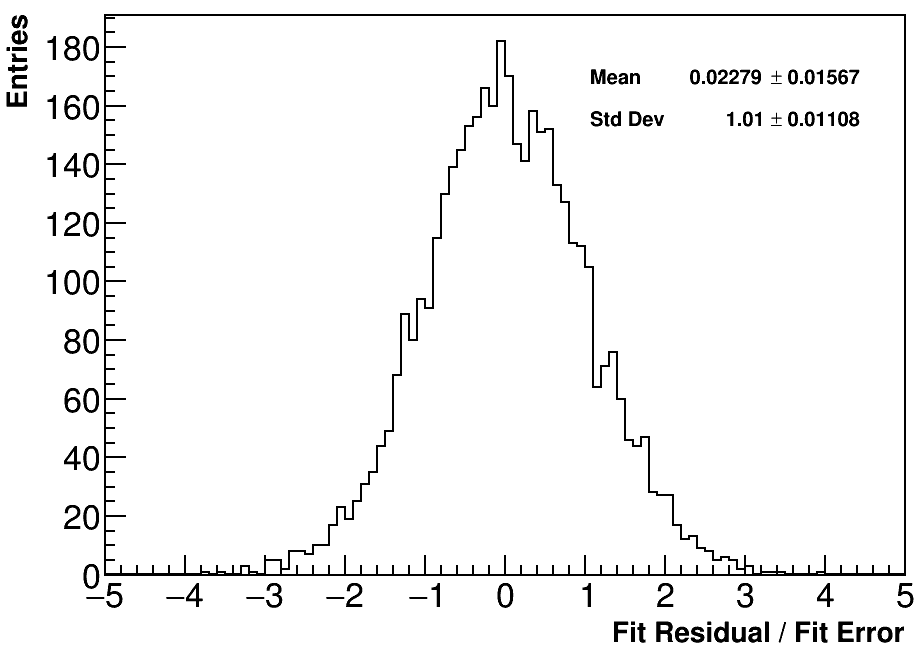
\includegraphics[width=\textwidth]{fitPull_projected_60h}
        % \caption{}
    \end{subfigure}
    % \hspace{5mm}
    \begin{subfigure}[b]{0.9\textwidth}
        \centering
        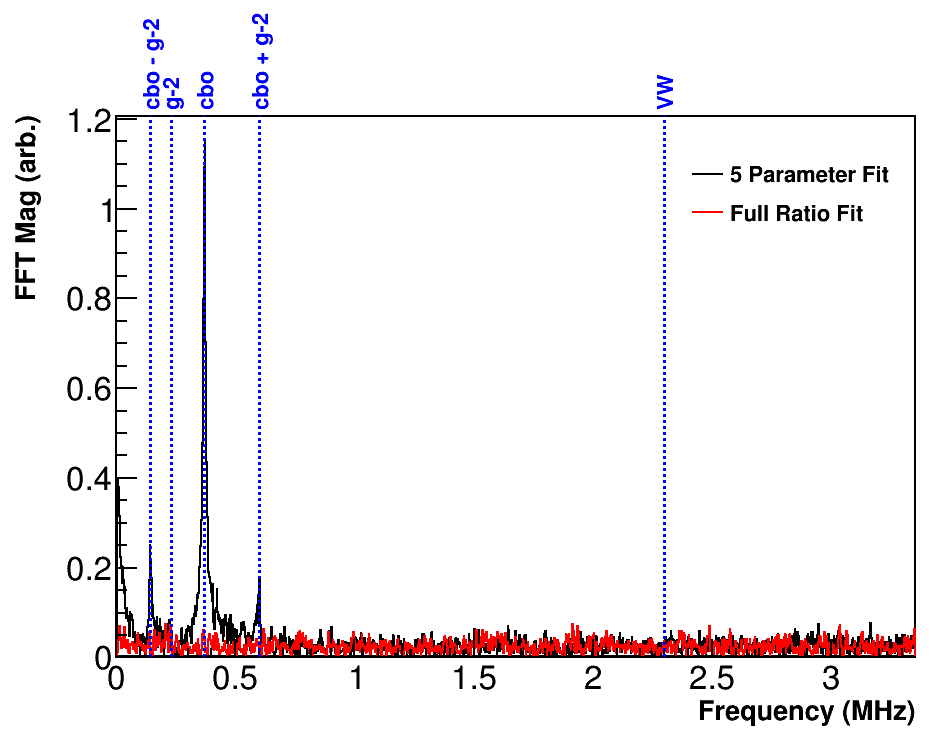
\includegraphics[width=\textwidth]{FFTComparison_FullRatio_60h}
        % \caption{}
        \vspace{3mm}
    \end{subfigure}
\caption[Pulls and FFT of residuals for the ratio fit to the 60h dataset]{Fit pulls (top-left), their projection on to the y axis (bottom-left), and the FFT of the fit residuals (right) for the ratio fit to the 60h dataset. Note the pull projection has a Gaussian shape centered around zero with unit width. In the FFT the results from a five parameter fit to the data are overlayed, along with blue dashed lines for the main beam dynamics peaks which appear in the data. There is no obvious structure in the pulls and no remaining peaks above the noise in the ratio fit FFT.}
\label{fig:fitResiduals_60h}
\end{figure}
\end{landscape}
% }


The CBO frequencies for the 60h and Endgame datasets with $n$ values of 0.108 were found to be 2.338 and 2.339 rad/\mus{} respectively, corresponding to approximately \SI{0.37}{MHz}. For the HighKick and 9d datasets with $n$ values of 0.120, the CBO frequencies were found to be 2.559 and 2.615 rad/\mus{} respectively, corresponding to approximately \SI{0.415}{MHz}. These frequencies correspond to the expected frequencies as described in \secref{sec:muonbeamdynamics}, with some slight deviations due to statistics, bad resistors, and the reduced sensitivity in the Ratio Method\footnote{The VW frequencies, though time-randomized out in the analysis presented here, were found to be approximately \SI{2.30}{} and \SI{2.04}{MHz} for the datasets with $n=0.108$ and $n=0.120$ respectively.}. The CBO lifetimes between the different datasets are relatively consistent, barring the HighKick dataset for which a smaller CBO lifetime was measured, attributed to the changing behavior of the bad resistors in that dataset. Ratio Method fits typically converge with lifetimes with large errors compared to T-Method fits, due to the reduction in sensitivity in the Ratio Method. In the HighKick dataset, the CBO lifetime did not like to converge nicely in the ratio fits, and was therefore fixed to that from a T-Method fit. The main CBO amplitudes $A_{cbo-N}$ for the different datasets were on the order of 0.3--0.4\%, while the higher order CBO amplitudes were in general an order of magnitude less. The strength of the various higher order CBO amplitudes fluctuated for different datasets, with one parameter being large compared to another in one dataset and vice versa in a different dataset. In some cases, the errors on the higher order CBO term amplitudes were of the order the amplitude itself. While this implies these terms can be dropped from the fit function, all terms were included for analysis uniformity among the different datasets. These relatively large errors, while making some of the fits slightly more challenging to achieve convergence, were nonetheless handled appropriately.



The final statistical errors on $R$ for the 60h, HighKick, 9d, and Endgame datasets are \SI{1.358}{}, \SI{1.411}{}, \SI{0.903}{}, and \SI{0.639}{ppm} respectively. The single seed $R$ results for the HighKick, 9d, and Endgame datasets, all of which used the same blinding string, are all well within $1\sigma$ of each other. The average $R$ value for fits to 50 different random seeds are provided in \secref{sub:randomSeedFits}.


Beyond looking at single fit residuals to evaluate the integrity of the fits, other checks were made to verify consistency. In general this consisted of slicing up the data in different ways and fitting the subsets. These tests and scans included fitting individual calorimeters, modifying the fit start and end times, adjusting the applied energy thresholds, and fitting individual beam bunches.





\clearpage

\subsection{Individual calorimeter fits}
\label{sub:per_calorimeter_fits}


Fits to all 24 individual calorimeters for each of the datasets were performed with the same number of free fit parameters as used in the calorimeter sum fits. \figref{fig:caloFits_chi2} shows the \chisq/NDF's for the calorimeter fits which are nicely spread around 1. \figref{fig:caloFits_R} shows the fitted $R$ values as a function of calorimeter number. Straight line fits were performed to the $R$ values with good \chisq's, and the fitted constant returned a value in each case that was consistent with the calorimeter sum fit $R$ values. Examining the $R$ values as a function of calorimeter between datasets, particular calorimeter numbers do not tend to lie above or below the fitted average. The spread in $R$ values for each calorimeter then can be said to be driven statistically, though it should be noted that with the larger error bars on the individual calorimeter fits it's hard to tell if there are any preferences one way or another.


\begin{figure}
\centering
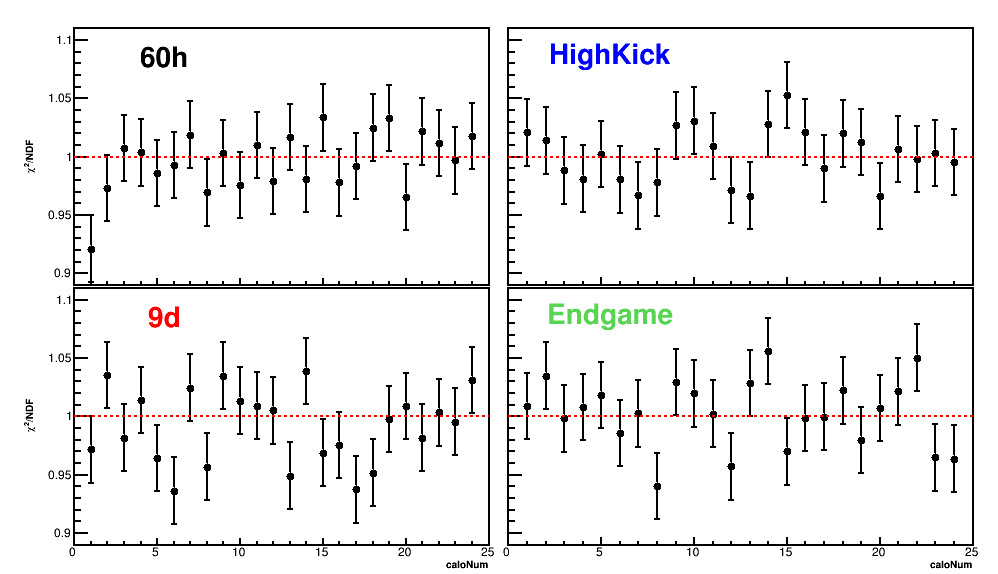
\includegraphics[width=0.84\linewidth]{caloFits_chi2_fourDatsets}
    \caption[\chisq/NDF versus calorimeter number]{\chisq/NDF versus calorimeter for the Run~1 precession frequency analysis datasets. Red dashed lines are placed at $\chi^{2}/\text{NDF} = 1$ to aid the eye. No individual calorimeter fits are preferentially low or high when comparing across datasets.}
    \label{fig:caloFits_chi2}
\vspace{4mm}
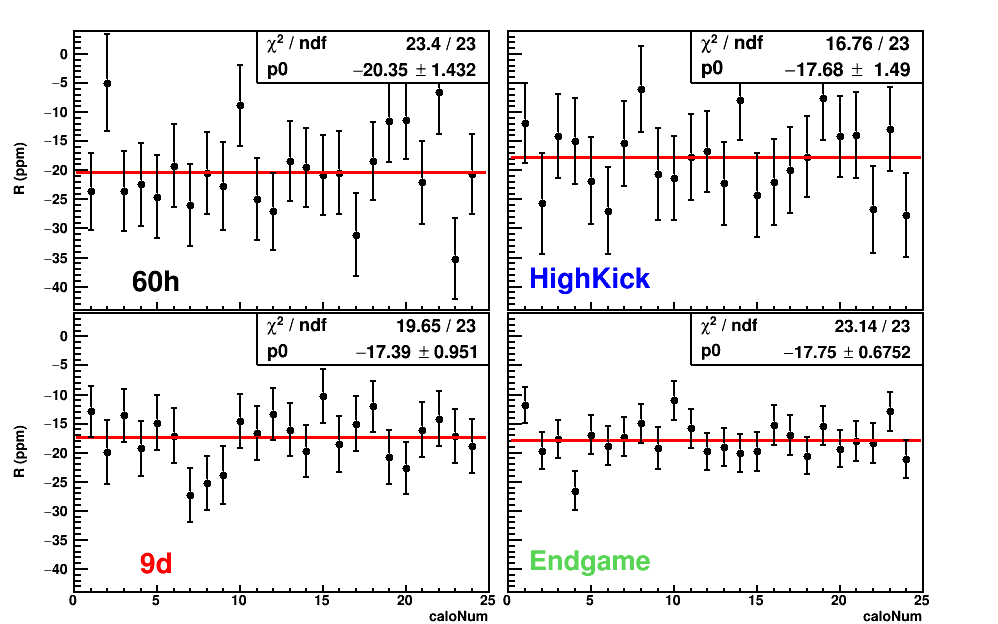
\includegraphics[width=0.84\linewidth]{caloFits_R_fourDatsets}
    \caption[$R$ versus calorimeter number]{$R$ versus calorimeter for the Run~1 precession frequency analysis datasets. The scale is the same on each of the plots.  A straight line fit was performed on the fitted values, with the fit result shown in the upper right box as parameter $p_{1}$ in units of ppm.The different blinding in the 60h dataset is readily observed, along with the higher precision fits in the 9d and Endgame datasets with their correspondingly smaller error bars.}
    \label{fig:caloFits_R}
\end{figure}


Figures~\ref{fig:caloFits_EndgamePars_1} and \ref{fig:fig:caloFits_EndgamePars_2} show calorimeter fit results for the other free parameters in the fit for the Endgame dataset. The \gmtwo phases are seen to be distinct among the different calorimeters, attributed to the different level of material upstream and therefore different acceptance. This is particularly noticeable in calorimeters 13 and 19 which sit behind the tracker stations. Any correlated effects on $R$ are not immediately observed, and might potentially be hidden behind the large errors of the fit. Similarly, the different calorimeters have different fit asymmetries, once again due to their different acceptances. The CBO parameters are in general consistent with some spread due to acceptance, with the phases running from 0--2$\pi$ around the ring as expected. As one might notice, the amplitudes of the CBO parameters are an order of magnitude higher than in the calorimeter sum fits. Because the phases vary around the ring, when adding up all the calorimeters the CBO effect becomes reduced. In fact, while it is not always necessary to include the higher order CBO terms for good fits to the calorimeter sum data, there are many calorimeters which need the higher order terms for good fits.


\begin{figure}
\centering
    \begin{subfigure}[]{0.45\textwidth}
        \centering
        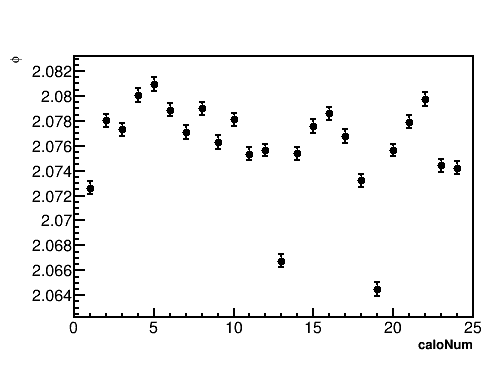
\includegraphics[width=\textwidth]{FullRatioFit_phi_Vs_Calo_Canv_Endgame}
        \caption{$\phi$}
    \end{subfigure}% %you need this % here to add spacing between subfigures
    \begin{subfigure}[]{0.45\textwidth}
        \centering
        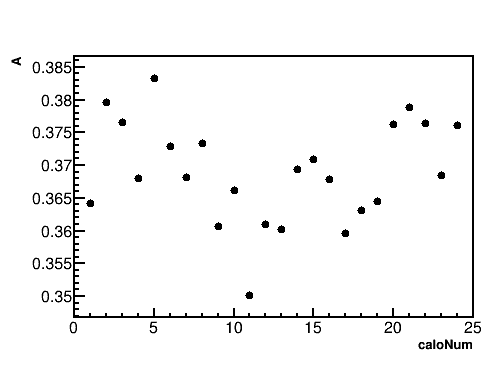
\includegraphics[width=\textwidth]{FullRatioFit_A_Vs_Calo_Canv_Endgame}
        \caption{$A$}
    \end{subfigure}

    \begin{subfigure}[]{0.45\textwidth}
        \centering
        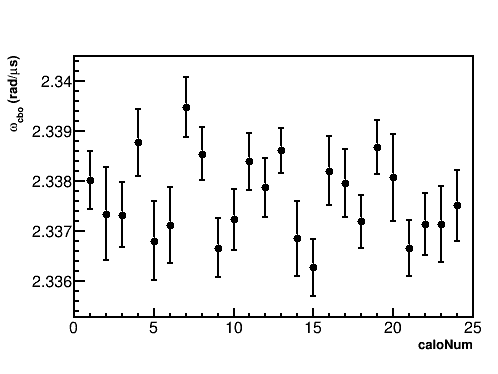
\includegraphics[width=\textwidth]{FullRatioFit_omega_cbo_Vs_Calo_Canv_Endgame}
        \caption{$\omega_{cbo}$}
    \end{subfigure}% %you need this % here to add spacing between subfigures
    \begin{subfigure}[]{0.45\textwidth}
        \centering
        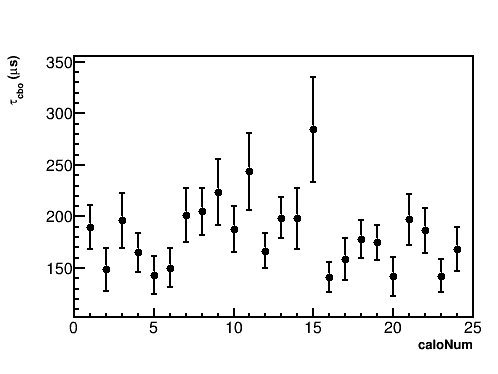
\includegraphics[width=\textwidth]{FullRatioFit_tau_cbo_Vs_Calo_Canv_Endgame}
        \caption{$\tau_{cbo}$}
    \end{subfigure}

    \begin{subfigure}[]{0.45\textwidth}
        \centering
        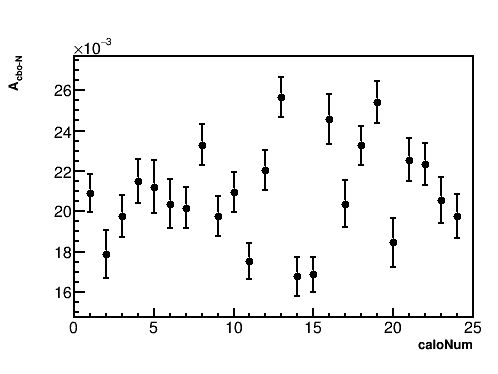
\includegraphics[width=\textwidth]{FullRatioFit_A_cbo-N_Vs_Calo_Canv_Endgame}
        \caption{$A_{cbo-N}$}
    \end{subfigure}% %you need this % here to add spacing between subfigures
    \begin{subfigure}[]{0.45\textwidth}
        \centering
        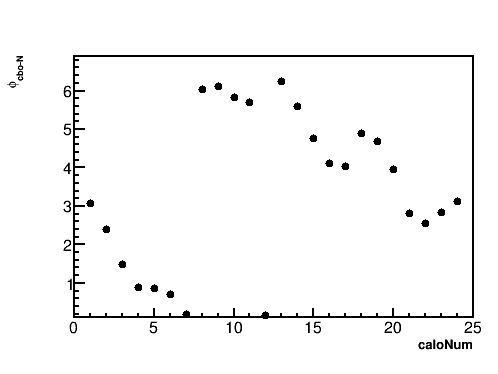
\includegraphics[width=\textwidth]{FullRatioFit_phi_cbo-N_Vs_Calo_Canv_Endgame}
        \caption{$\phi_{cbo-N}$}
    \end{subfigure}
\caption[Endgame fit parameters versus calorimeter number]{Endgame fit parameters versus calorimeter number. In the  \gmtwo phase $\phi$ (top-left) two points lie below the others, corresponding to those calorimeters which sit behind tracker stations. The CBO phase $\phi_{cbo-N}$ (bottom-right) runs from 0--2$\pi$ around the ring. These plots are typical of all datasets, with small variations in the final fitted parameters.}
\label{fig:caloFits_EndgamePars_1}
\end{figure}

\begin{figure}
\centering
    \begin{subfigure}[]{0.45\textwidth}
        \centering
        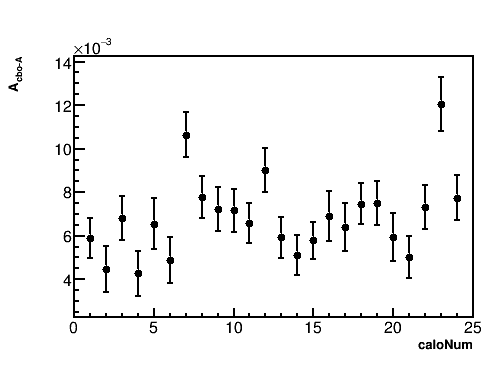
\includegraphics[width=\textwidth]{FullRatioFit_A_cbo-A_Vs_Calo_Canv_Endgame}
        \caption{$A_{cbo-A}$}
    \end{subfigure}% %you need this % here to add spacing between subfigures
    \begin{subfigure}[]{0.45\textwidth}
        \centering
        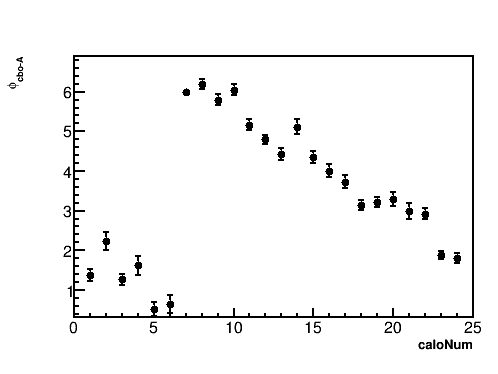
\includegraphics[width=\textwidth]{FullRatioFit_phi_cbo-A_Vs_Calo_Canv_Endgame}
        \caption{$\phi_{cbo-A}$}
    \end{subfigure}

    \begin{subfigure}[]{0.45\textwidth}
        \centering
        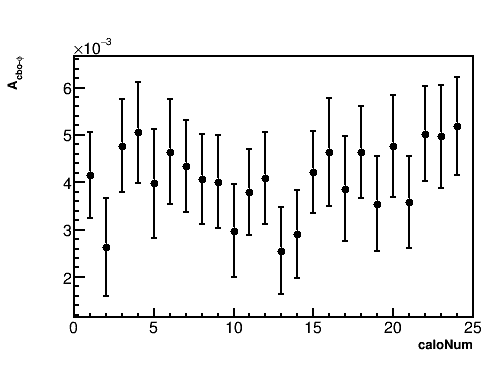
\includegraphics[width=\textwidth]{FullRatioFit_A_cbo-phi_Vs_Calo_Canv_Endgame}
        \caption{$A_{cbo-\phi}$}
    \end{subfigure}% %you need this % here to add spacing between subfigures
    \begin{subfigure}[]{0.45\textwidth}
        \centering
        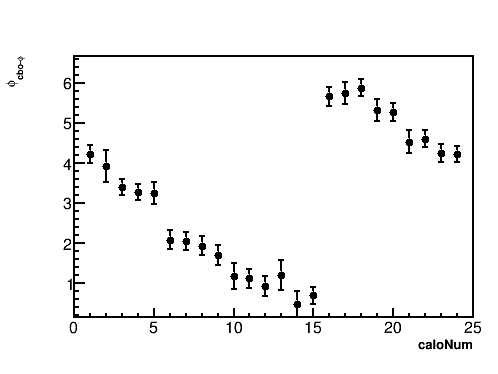
\includegraphics[width=\textwidth]{FullRatioFit_phi_cbo-phi_Vs_Calo_Canv_Endgame}
        \caption{$\phi_{cbo-\phi}$}
    \end{subfigure}

    \begin{subfigure}[]{0.45\textwidth}
        \centering
        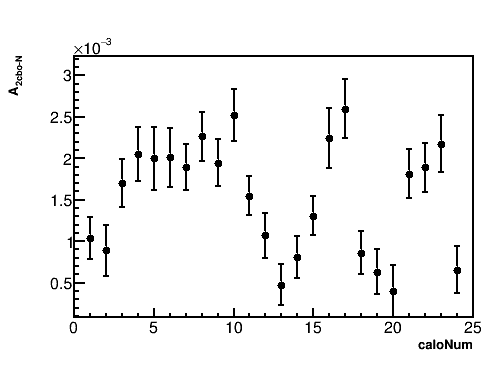
\includegraphics[width=\textwidth]{FullRatioFit_A_2cbo-N_Vs_Calo_Canv_Endgame}
        \caption{$A_{2cbo-N}$}
    \end{subfigure}% %you need this % here to add spacing between subfigures
    \begin{subfigure}[]{0.45\textwidth}
        \centering
        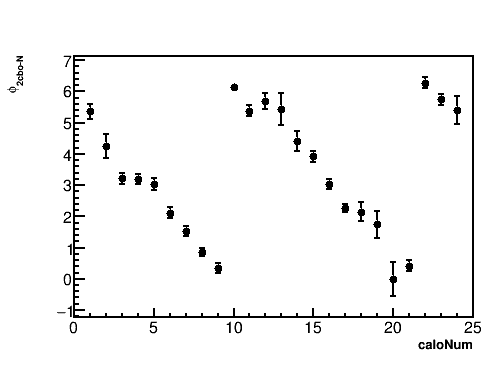
\includegraphics[width=\textwidth]{FullRatioFit_phi_2cbo-N_Vs_Calo_Canv_Endgame}
        \caption{$\phi_{2cbo-N}$}
    \end{subfigure}
\caption[Endgame fit parameters versus calorimeter number]{Endgame fit parameters versus calorimeter number. The CBO phases $\phi_{cbo-A}$ and $\phi_{cbo-\phi}$ run from 0--2$\pi$ around the ring, while $\phi_{2cbo-N}$ runs around twice. These plots are typical of all datasets, with small variations in the final fitted parameters.}
\label{fig:fig:caloFits_EndgamePars_2}
\end{figure}


\clearpage

\subsection{Fit start and end scans}


In order to determine if there are any deficiencies as a function of time, for instance if the CBO was modeled incorrectly, fits are performed with varying fit start and end times. If a parameter is incorrectly modeled, it will wander away from the statistically allowed deviation as the mis-modeled effect grows stronger or weaker. Two examples of this are given in \figref{fig:badStartScans}. In the first case the CBO frequency was mis-measured when excluding the changing CBO frequency model, and in the second case the asymmetry was mis-measured when pileup was not subtracted from the data. In general, doing a fit start scan is a very useful tool in the precession frequency analysis beyond just verifying consistency of a fit parameter as a function of time, as it also provides hints as to what might be wrong with how the data is being handled.


\begin{figure}
\centering
    \begin{subfigure}[t]{0.45\textwidth}
        \centering
        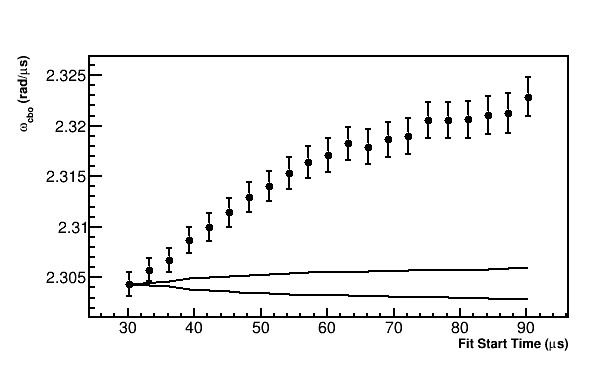
\includegraphics[width=\textwidth]{FullRatio_omega_cbo_FS_Canv_Endgame_fixedCBOModel}
        \caption{The fit start scan for the fitted CBO frequency when a constant frequency model is included. The p-value of the first ratio fit in this case is 0.191, indicating an acceptable fit. Only by performing a fit start scan or examining the fit residuals closely is the deficiency in the fit observed.}
    \end{subfigure}% %you need this % here to add spacing between subfigures
    \hspace{4mm}
    \begin{subfigure}[t]{0.45\textwidth}
        \centering
        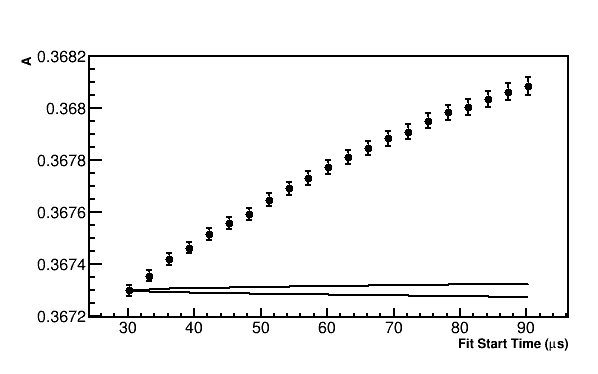
\includegraphics[width=\textwidth]{FullRatio_A_FS_Canv_Endgame_noPileupSubraction}
        \caption{The fit start scan for the fitted asymmetry when the pileup is not subtracted out. If the pileup is not properly accounted for, then decay positrons with lower asymmetries contaminate the observed decay time spectrum leading to a lower fitted asymmetry value. As the pileup diminishes the fitted asymmetry tends to it's true value.}
    \end{subfigure}
\caption[Examples of fit start scans when effects are improperly accounted for in fitting]{Examples of fit start scans when effects are improperly accounted for in fitting. The parabolic bands indicate the one sigma allowed deviation in the fit parameters due to the changing statistics between the fits. Data are from the Endgame dataset.}
\label{fig:badStartScans}
\end{figure}



The statistically allowed deviation between two sets of \gmtwo data, where one is a subset of the other, is given by \cite{E821FinalReport}
  \begin{align} \label{eq:sigmaDiffFull}
    \sigma_{diff} = \sqrt{\sigma_{2} - \sigma_{1}(2 \frac{A_{1}}{A_{2}}\cos(\phi_{1}-\phi_{2}) - 1)},
  \end{align}
where the subscript 2 stands for the larger dataset while the subscript 1 stands for the smaller sub-dataset. This statistically allowed deviation depends both on the size of the datasets as well as their ``analyzing powers,'' which come from the asymmetries and phases of the datasets. For fit start scans the analyzing powers are in general the same, such that the approximation 
  \begin{align} \label{eq:sigmaDiffApprox}
    \sigma_{diff} \approx \sqrt{\sigma_{2} - \sigma_{1}}
  \end{align}
can be made. 


It should be noted that for fits with late fit start times, certain CBO parameters start to become unstable as the CBO effect becomes diminished in the data\footnote{The same applies to the VW effect when it is not time-randomized out of the data.}. Fits with start times at \mus{100} are half a lifetime or more along the CBO effect and convergence is difficult to achieve. For those parameters which were found to be unreliable, they were fixed to their starting fit values. These typically included the CBO lifetime and most of the higher order CBO amplitudes and phases, though in some cases they could still be included out to late fit start times depending on the dataset.


Fit start time scans were performed from the default value of \mus{30.2} up to \mus{100.2} in steps of \mus{1} corresponding to 71 separate fits. In order to assist fit convergence, the final fit parameters from one fit were passed on as the starting parameters of the next. The \chisq/NDF's and fitted $R$ values as a function of fit start time for the four Run~1 precession frequency analysis datasets are shown in \figref{fig:fitStartTime_chi2_and_R}. The error on the individual points in the \chisq plots are given as 
  \begin{align}
    \sigma_{\chi^{2}/NDF} = \sqrt{2/NDF},
  \end{align}
where NDF changes as the fit start time is pushed later in time and bins are left out of the fit. The black parabolic bands indicate the $1\sigma$ statistically allowed deviation as given by \equref{eq:sigmaDiffApprox}. As shown the goodness of fit for the four datasets are all consistent with fit start time, only wandering in and near the bands without diverging.


$R$ is similarly consistent as a function of fit start time. The only dataset for which $R$ goes noticeably outside the bands more than the others is that for the HighKick. Since the deviation is less than $2\sigma$ and it appears to have a trend back towards the bands however, it does not appear particularly indicative of unaccounted effects in the data. In general $R$ is very insensitive to changing fit start time, most likely due to the small correlations with other fit parameters.


\figref{fig:fitStartScan_EndgamePars} shows the fit start scan results for the other free parameters for the Endgame dataset. In all cases the fit parameters only wander in and near the bands, showing that all effects in the ratio data are properly accounted for.


\begin{landscape}
\begin{figure}
    \centering
    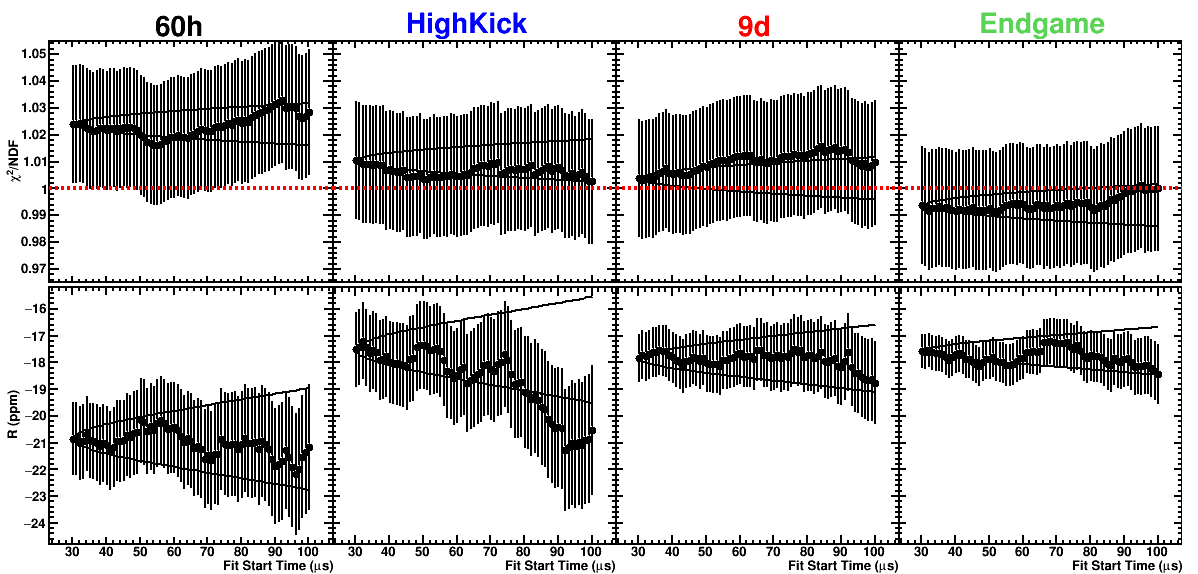
\includegraphics[width=1\linewidth]{fitStartScan_R_fourDatasets}
    \caption[\chisq/NDF and $R$ versus fit start time]{\chisq/NDF (top) and $R$ (bottom) versus fit start time for the Run~1 precession frequency analysis datasets. Plots in the top and bottom rows are on the same scale respectively. The black parabolic bands represent the $1\sigma$ statistically allowed deviation. The \chisq values are all consistent with 1, for which a dashed red line has been overlayed. In all cases the fit points lie in and around the $1\sigma$ statistical bands.}
    \label{fig:fitStartTime_chi2_and_R}
\end{figure}
\end{landscape}


\begin{figure}
\centering
    \begin{subfigure}[]{0.45\textwidth}
        \centering
        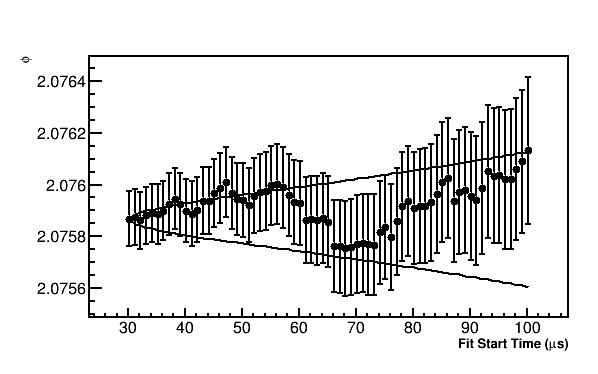
\includegraphics[width=\textwidth]{FullRatio_phi_FS_Canv_Endgame}
        \caption{$\phi$}
    \end{subfigure}% %you need this % here to add spacing between subfigures
    \begin{subfigure}[]{0.45\textwidth}
        \centering
        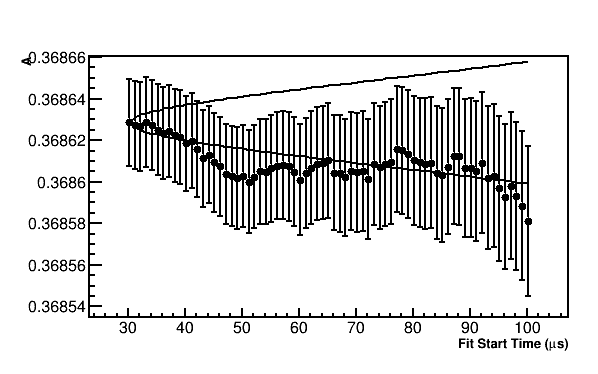
\includegraphics[width=\textwidth]{FullRatio_A_FS_Canv_Endgame}
        \caption{$A$}
    \end{subfigure}

    \begin{subfigure}[]{0.45\textwidth}
        \centering
        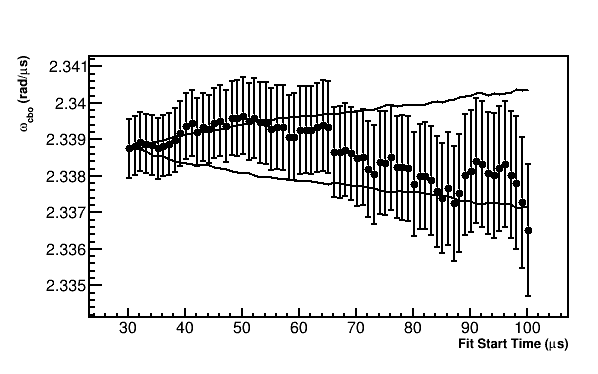
\includegraphics[width=\textwidth]{FullRatio_omega_cbo_FS_Canv_Endgame}
        \caption{$\omega_{cbo}$}
    \end{subfigure}% %you need this % here to add spacing between subfigures
    \begin{subfigure}[]{0.45\textwidth}
        \centering
        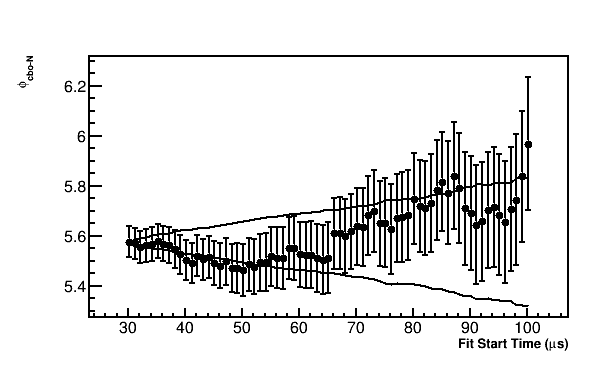
\includegraphics[width=\textwidth]{FullRatio_phi_cbo-N_FS_Canv_Endgame}
        \caption{$\phi_{cbo-N}$}
    \end{subfigure}

    \begin{subfigure}[]{0.45\textwidth}
        \centering
        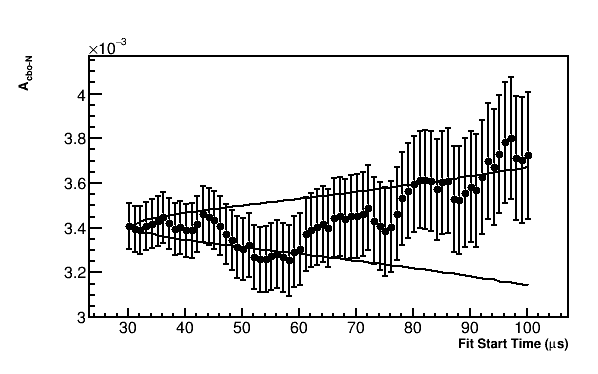
\includegraphics[width=\textwidth]{FullRatio_A_cbo-N_FS_Canv_Endgame}
        \caption{$A_{cbo-N}$}
    \end{subfigure}% %you need this % here to add spacing between subfigures
    \begin{subfigure}[]{0.45\textwidth}
        \centering
        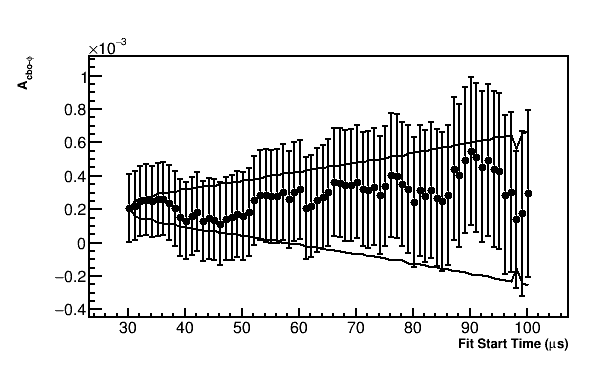
\includegraphics[width=\textwidth]{FullRatio_A_cbo-phi_FS_Canv_Endgame}
        \caption{$A_{cbo-\phi}$}
    \end{subfigure}
\caption[Fit start scans for free parameters in the Endgame dataset]{Fit start scans for free parameters in the Endgame dataset. Those parameters not shown here are fixed to their starting values over the course of the scan, as at late times they can be unstable as the CBO effects die away.}
\label{fig:fitStartScan_EndgamePars}
\end{figure}


For fit end scans, all of the same methods and conclusions apply. In general fit end scans are both less dangerous and more stable than fit start scans, as the amount of data being removed from the fit is relatively small. While these fit end scans in a T-Method fit might be able to be completely ignored in favor of the fit start scans, it's important to check that they satisfy the statistical deviations in the Ratio Method as the ratio data errors grow larger with less data \cite{BU60hReport}. Fit end time scans were performed from \mus{650} to \mus{400} in steps of \mus{10}, corresponding to 26 separate fits. As in the fit start time scan, fit results from the end of one fit were passed on as the starting parameters to the next. $R$ values for fit end scans for the Run~1 precession frequency analysis datasets are shown in \figref{fig:fitEndTime_R}. As shown the $R$ values are comfortably within and near the bands.


\begin{figure}
\centering
    \begin{subfigure}[]{0.45\textwidth}
        \centering
        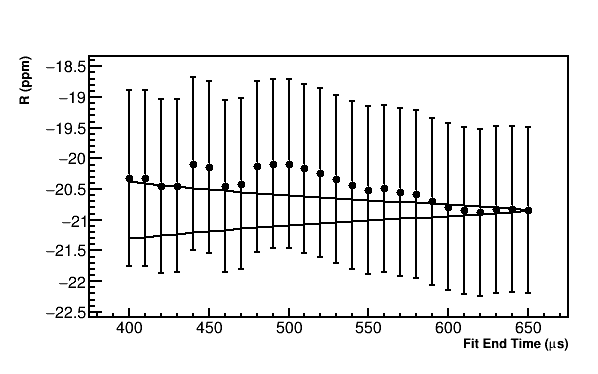
\includegraphics[width=\textwidth]{FullRatio_R_FE_Canv_60h}
        \caption{60h dataset.}
    \end{subfigure}% %you need this % here to add spacing between subfigures
    \begin{subfigure}[]{0.45\textwidth}
        \centering
        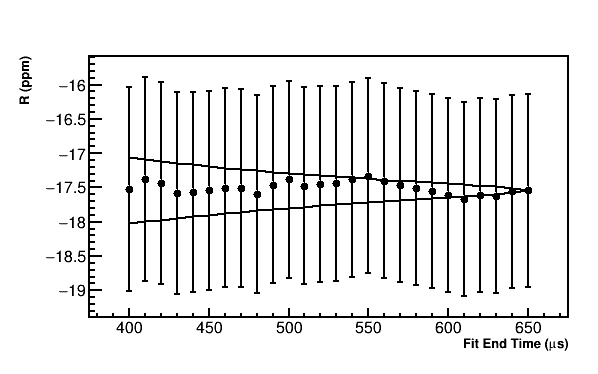
\includegraphics[width=\textwidth]{FullRatio_R_FE_Canv_HighKick}
        \caption{HighKick dataset.}
    \end{subfigure}

    \begin{subfigure}[]{0.45\textwidth}
        \centering
        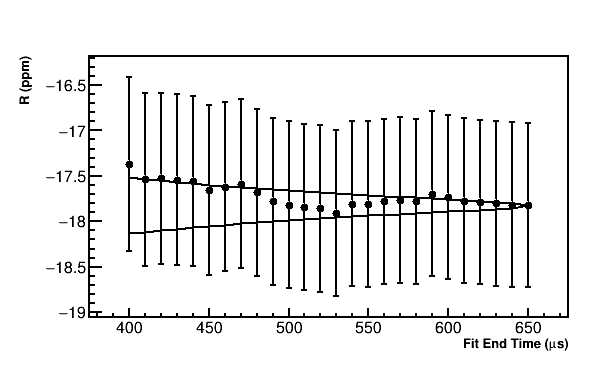
\includegraphics[width=\textwidth]{FullRatio_R_FE_Canv_9d}
        \caption{9d dataset.}
    \end{subfigure}% %you need this % here to add spacing between subfigures
    \begin{subfigure}[]{0.45\textwidth}
        \centering
        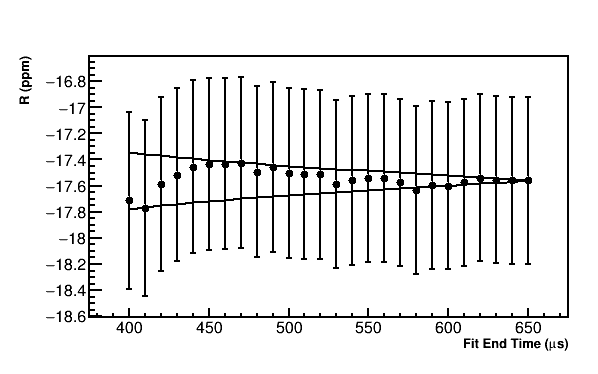
\includegraphics[width=\textwidth]{FullRatio_R_FE_Canv_Endgame}
        \caption{Endgame dataset.}
    \end{subfigure}
\caption[$R$ versus fit end time]{$R$ versus fit end time for the Run~1 precession frequency analysis datasets. The fit points lie in and around the $1\sigma$ statistical bands.}
\label{fig:fitEndTime_R}
\end{figure}

\clearpage 

\subsection{Energy threshold scans}


Similarly to fit start and end time scans, it is worthwhile to verify that $R$ is consistent regardless of the energy threshold applied to the decay positron time spectrum. The energy threshold was varied from \SI{1.2}{\GeV} to \SI{2.2}{\GeV} in steps of \SI{50}{\MeV} corresponding to 21 separate fits. The fitted $R$ values for the four Run~1 precession frequency analysis datasets are shown in \figref{fig:energyThresholdScan_R}. The statistical bands are the same as those defined in \equref{eq:sigmaDiffFull}, where now the analyzing power part of the equation plays a larger role as the asymmetries and phases of the different fit points are significantly different. As shown there are no major deviations in the fitted $R$ values.


\begin{figure}
\centering
    \begin{subfigure}[]{0.45\textwidth}
        \centering
        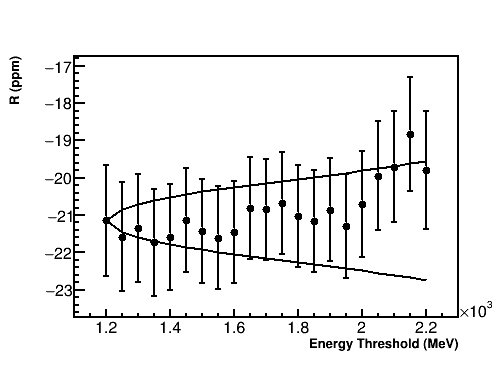
\includegraphics[width=\textwidth]{FullRatio_R_Vs_ETh_60h}
        \caption{60h dataset.}
    \end{subfigure}% %you need this % here to add spacing between subfigures
    \begin{subfigure}[]{0.45\textwidth}
        \centering
        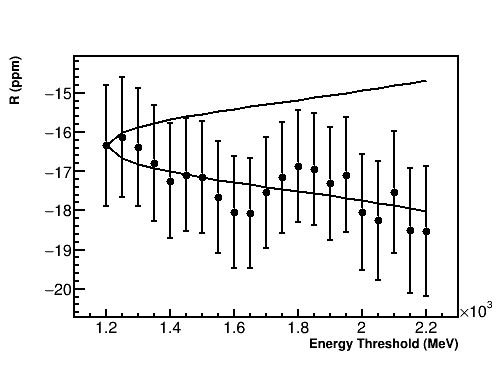
\includegraphics[width=\textwidth]{FullRatio_R_Vs_ETh_HighKick}
        \caption{HighKick dataset.}
    \end{subfigure}

    \begin{subfigure}[]{0.45\textwidth}
        \centering
        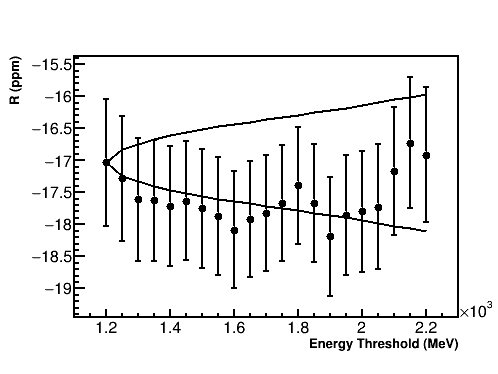
\includegraphics[width=\textwidth]{FullRatio_R_Vs_ETh_9d}
        \caption{9d dataset.}
    \end{subfigure}% %you need this % here to add spacing between subfigures
    \begin{subfigure}[]{0.45\textwidth}
        \centering
        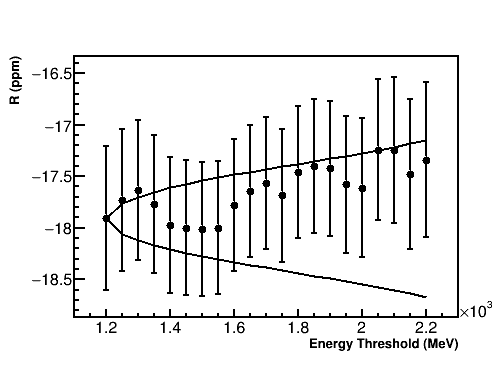
\includegraphics[width=\textwidth]{FullRatio_R_Vs_ETh_Endgame}
        \caption{Endgame dataset.}
    \end{subfigure}
\caption[$R$ versus energy threshold]{$R$ versus energy threshold for the Run~1 precession frequency analysis datasets. The fit points lie in and around the $1\sigma$ statistical bands.}
\label{fig:energyThresholdScan_R}
\end{figure}



\clearpage


\subsection{Fits to bunch number}


As described in \secref{sec:Accelerator}, eight distinct and separate bunches of muons are sent to the E989 experiment within the accelerator timing structure. Differences upstream and at injection mean that the stored beam is slightly different between the bunches. In order to verify that the treatment of fit parameters was correct regardless of the bunch number and improve confidence in the results, the bunches were fit individually. \figref{fig:bunchNum_R} shows the fitted $R$ values for the eight individual bunches alongside the bunch-sum result, for the Run~1 precession frequency analysis datasets. In all cases there appear no systematically different $R$ values per bunch. When the eight individual bunches were fit to a straight line, they were found to be consistent with the bunch-sum result.


% If different bunches have different momentum spreads due to how the particles are transported down the various beamlines and injected into the storage ring, then muons might live for different times and therefore their spins might precess more or less within the magnetic field. This difference in \gmtwo phase between the different bunches would then affect the final fitted $R$ value, and might be a systematic error in the precession frequency measurement if certain bunches have significantly more statistics than the others. <- wrong


\begin{figure}
\centering
    \begin{subfigure}[]{0.45\textwidth}
        \centering
        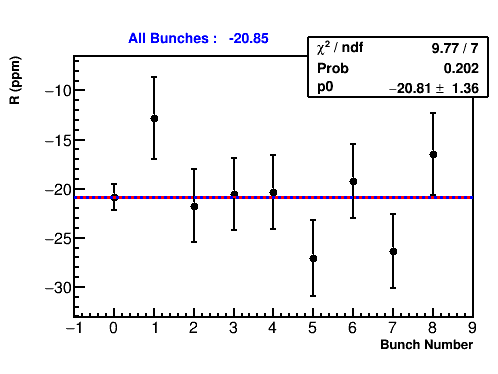
\includegraphics[width=\textwidth]{FullRatio_R_Vs_BunchNum_Canv_60h}
        \caption{60h dataset.}
    \end{subfigure}% %you need this % here to add spacing between subfigures
    \begin{subfigure}[]{0.45\textwidth}
        \centering
        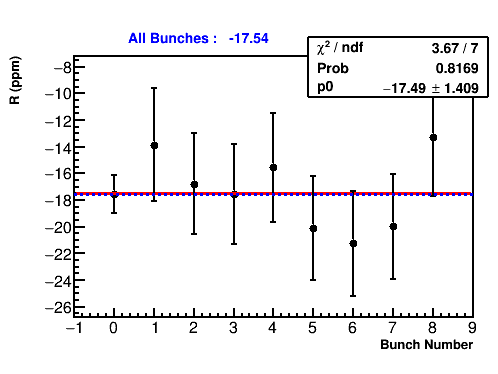
\includegraphics[width=\textwidth]{FullRatio_R_Vs_BunchNum_Canv_HighKick}
        \caption{HighKick dataset.}
    \end{subfigure}

    \begin{subfigure}[]{0.45\textwidth}
        \centering
        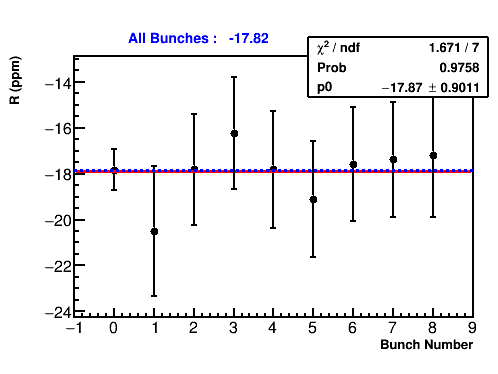
\includegraphics[width=\textwidth]{FullRatio_R_Vs_BunchNum_Canv_9d}
        \caption{9d dataset.}
    \end{subfigure}% %you need this % here to add spacing between subfigures
    \begin{subfigure}[]{0.45\textwidth}
        \centering
        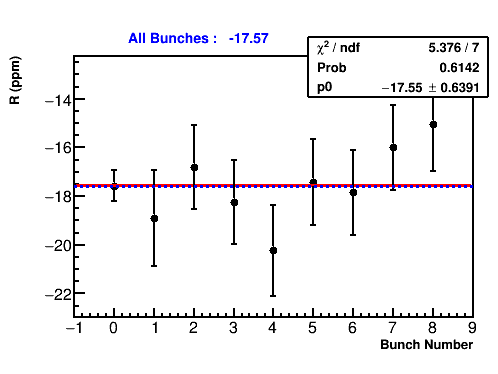
\includegraphics[width=\textwidth]{FullRatio_R_Vs_BunchNum_Canv_Endgame}
        \caption{Endgame dataset.}
    \end{subfigure}
\caption[$R$ versus bunch number]{$R$ versus bunch number for the Run~1 precession frequency analysis datasets. Bunch number 0 corresponds to the data from all bunches added together. The blue dashed line intersects the bunch number 0 point, and it's value is displayed in the top left of each plot. The red line corresponds to a fit to bunches 1--8, with $p_{0}$ being the fit parameter. In all cases the fitted $R$ value to bunches 1--8 is nearly identical to the all-bunches result.}
\label{fig:bunchNum_R}
\end{figure}


\clearpage


\subsection{Fits to many random seeds}
\label{sub:randomSeedFits}


While the single seed fit results presented earlier indicate good fits and well understood parameters, it is always a good idea to fit other random seeds in case the single seed results ended up on an outlier. Doing so not only improves the confidence of the result, but also gives a more central $R$ value to quote as being closer to the `true' $R$ of the dataset. Figures~\ref{fig:randomSeedFits_chi2} and \ref{fig:randomSeedFits_R} give the \chisq and $R$ distributions for fits to 50 different random seeds for the four datasets. As shown the \chisq distributions are centered around 1 as expected. \tabref{tab:RandomSeedFitResults} compares the random seed fit results between the different datasets. The means for the $R$ distributions of the datasets which shared the same blinding string (HighKick, 9d, Endgam) are statistically consistent with one another, with differences on the order of several hundreds of ppb, well within the statistical errors of \SI{600}{ppb} or greater\footnote{The errors on the mean are calculated as $\sigma_{\mu} = \text{RMS}/\sqrt{N},$ where $N$ is the number of random seeds. These errors come from the randomization of cluster times before fitting, and have no bearing on statistical consistency when comparing different datasets.}.



\begin{figure}
\centering
    \begin{subfigure}[]{0.45\textwidth}
        \centering
        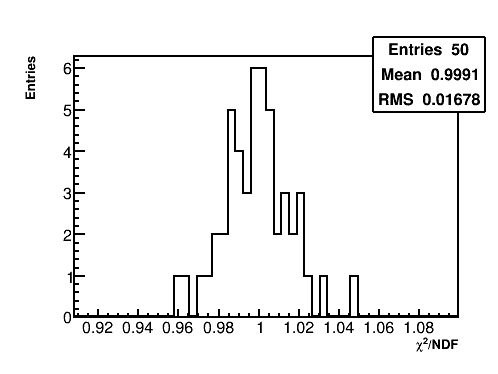
\includegraphics[width=\textwidth]{FullRatio_Chi2NDF_Vs_Iter_Canv_hist_60h}
        \caption{60h dataset.}
    \end{subfigure}% %you need this % here to add spacing between subfigures
    \begin{subfigure}[]{0.45\textwidth}
        \centering
        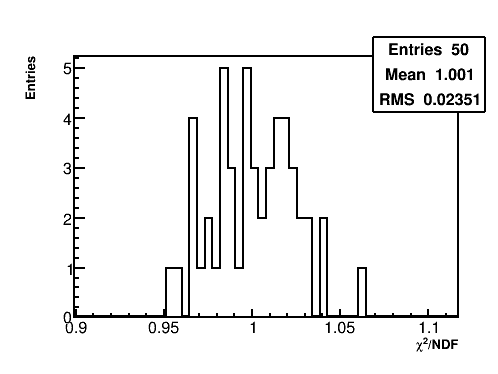
\includegraphics[width=\textwidth]{FullRatio_Chi2NDF_Vs_Iter_Canv_hist_HighKick}
        \caption{HighKick dataset.}
    \end{subfigure}

    \begin{subfigure}[]{0.45\textwidth}
        \centering
        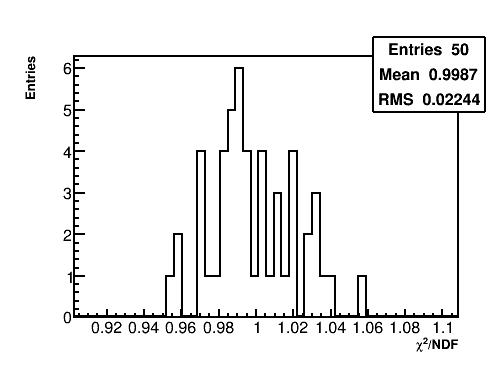
\includegraphics[width=\textwidth]{FullRatio_Chi2NDF_Vs_Iter_Canv_hist_9d}
        \caption{9d dataset.}
    \end{subfigure}% %you need this % here to add spacing between subfigures
    \begin{subfigure}[]{0.45\textwidth}
        \centering
        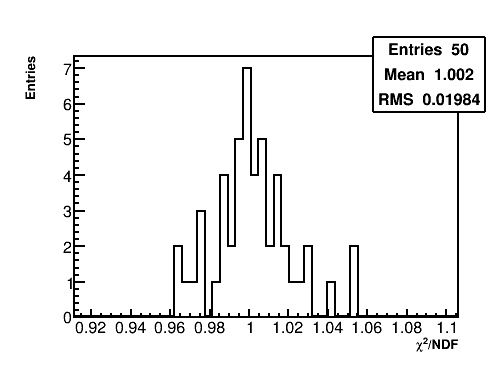
\includegraphics[width=\textwidth]{FullRatio_Chi2NDF_Vs_Iter_Canv_hist_Endgame}
        \caption{Endgame dataset.}
    \end{subfigure}
\caption[\chisq's for fits to many random seeds]{\chisq values for fits to 50 different random seeds for the Run~1 precession frequency analysis datasets. The distributions are nicely centered around 1 which is to be expected if the randomized data is properly distributed and fit correctly.}
\label{fig:randomSeedFits_chi2}
\end{figure}


\begin{figure}
\centering
    \begin{subfigure}[]{0.45\textwidth}
        \centering
        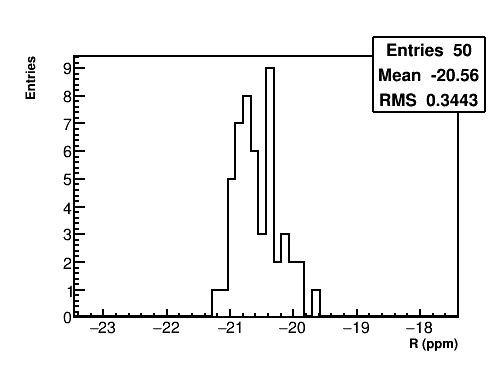
\includegraphics[width=\textwidth]{FullRatio_R_Vs_Iter_Canv_hist_60h}
        \caption{60h dataset.}
    \end{subfigure}% %you need this % here to add spacing between subfigures
    \begin{subfigure}[]{0.45\textwidth}
        \centering
        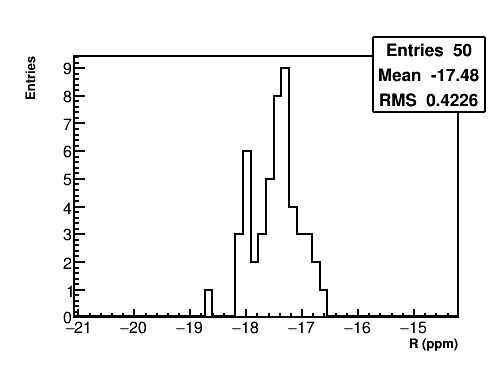
\includegraphics[width=\textwidth]{FullRatio_R_Vs_Iter_Canv_hist_HighKick}
        \caption{HighKick dataset.}
    \end{subfigure}

    \begin{subfigure}[]{0.45\textwidth}
        \centering
        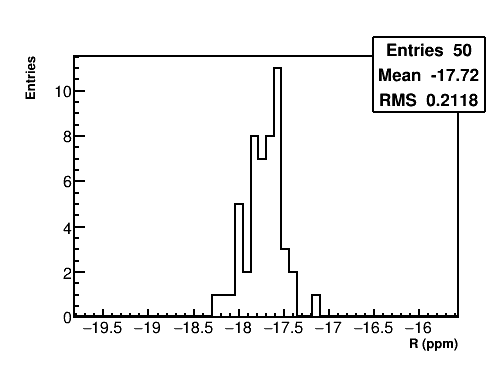
\includegraphics[width=\textwidth]{FullRatio_R_Vs_Iter_Canv_hist_9d}
        \caption{9d dataset.}
    \end{subfigure}% %you need this % here to add spacing between subfigures
    \begin{subfigure}[]{0.45\textwidth}
        \centering
        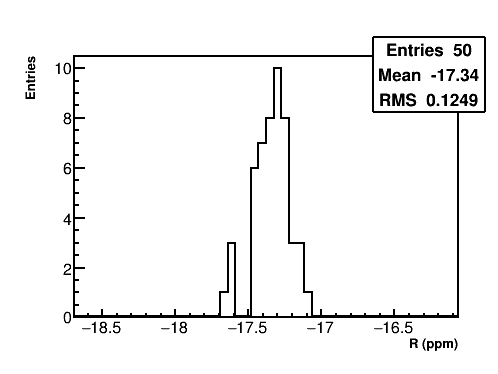
\includegraphics[width=\textwidth]{FullRatio_R_Vs_Iter_Canv_hist_Endgame}
        \caption{Endgame dataset.}
    \end{subfigure}
\caption[$R$ values for fits to many random seeds]{$R$ values for fits to 50 different random seeds for the Run~1 precession frequency analysis datasets. The statistics box has units of ppm for the mean and RMS of the distributions.}
\label{fig:randomSeedFits_R}
\end{figure}



\begin{table}
\centering
% \small
% \setlength\tabcolsep{10pt}
\renewcommand{\arraystretch}{1.2}
\begin{tabular*}{\linewidth}{@{\extracolsep{\fill}}lcccc}
  \hline
    \multicolumn{5}{c}{\textbf{Random Seed Fit Results}} \\
  \hline\hline
    Dataset & \chisq Mean & $R$ Mean & $R$ RMS & $R$ Error on Mean \\
  \hline
    60h & 0.999 & $-20.5562$ & 0.3443 & 0.0487 \\
    HighKick & 1.001 & $-17.4755$ & 0.4226 & 0.0598 \\
    9d & 0.999 & $-17.7182$ & 0.2118 & 0.0300 \\
    Endgame & 1.002 & $-17.3406$ & 0.1249 & 0.0177 \\
  \hline
\end{tabular*}
\caption[Random seed fit results]{Random seed fit results to the four Run~1 precession frequency analysis datasets. The \chisq means are consistent with 1. As a reminder the 60h dataset used a different blinding than the other three, hence the significantly different $R$ mean. Units are in ppm.}
\label{tab:RandomSeedFitResults}
\end{table}




% \begin{figure}
%     \centering
%     \includegraphics[width=.8\textwidth]{}
%     \caption[]{Data from some dataset.}
%     \label{fig:}
% \end{figure}

% \begin{figure}
% \centering
%     \begin{subfigure}[]{0.8\textwidth}
%         \centering
%         \includegraphics[width=\textwidth]{}
%         \caption{}
%     \end{subfigure}% %you need this % here to add spacing between subfigures
%     \vspace{1cm}
%     \begin{subfigure}[]{0.8\textwidth}
%         \centering
%         \includegraphics[width=\textwidth]{}
%         \caption{}
%     \end{subfigure}
% \caption[]{Data from some dataset.}
% \label{fig:}
% \end{figure}

% \begin{figure}
% \centering
%     \begin{subfigure}[]{0.45\textwidth}
%         \centering
%         \includegraphics[width=\textwidth]{}
%         \caption{}
%     \end{subfigure}% %you need this % here to add spacing between subfigures
%     \begin{subfigure}[]{0.45\textwidth}
%         \centering
%         \includegraphics[width=\textwidth]{}
%         \caption{}
%     \end{subfigure}

%     \begin{subfigure}[]{0.45\textwidth}
%         \centering
%         \includegraphics[width=\textwidth]{}
%         \caption{}
%     \end{subfigure}% %you need this % here to add spacing between subfigures
%     \begin{subfigure}[]{0.45\textwidth}
%         \centering
%         \includegraphics[width=\textwidth]{}
%         \caption{}
%     \end{subfigure}
% \caption[]{Data from some dataset.}
% \label{fig:}
% \end{figure}
